\documentclass[12pt]{article}
\usepackage{hyperref,graphicx}
\pagestyle{empty}
\textwidth=16.5cm
\textheight=21.0cm
\oddsidemargin=0cm
\topmargin=-0.5cm
\title{\vspace*{-1.5cm}
The new Classic ADS}
\author{A. Jabberwocky\footnote{email: jabberwocky-ads@protonmail.com}}
\date{August 1, 2019}
\begin{document}
\maketitle
\thispagestyle{empty}

\begin{abstract}
NASA ADS  underwent a major redesign in recent years, with the modern Javascript-based user interface replacing the older ``classic'' ADS, which will be closed down in a couple of months.
We introduce a ``neo-Classical'' interface for ADS, which allows one to perform some of the most commonly used tasks and display results in a familiar form, as a pure HTML webpage. It is available at \url{http://adsabs.net} and complements the official, more powerful modern web interface at \url{http://ui.adsabs.harvard.edu}.
\end{abstract}

NASA Astrophysics Data System (ADS) \cite{ADS} is an online bibliographic database and reference search engine for astronomical and physics literature. Conceived in early 1990s, around the same time as arXiv, it became an enormously valuable and an almost indispensable tool in everyday life of an average astronomer.

Over most of its lifetime, ADS provided a simple form-based user interface for searching papers, viewing abstracts and retrieving references and citations. Recently, the architecture of the system underwent a major redesign, separating the search engine from the user interface and providing an public API for querying the database programmatically \cite{ADS2}. The new user interface \cite{ADSnew}, codenamed \textsc{Bumblebee}, is written in JavaScript, uses modern web technologies, and provides a more interactive experience, even showing previews of paper figures and visualizations of citation statistics in a side panel. At the same time, it is also more resource-demanding, slow to load, and does not work at all in old web browsers. 
%By contrast, arXiv keeps almost the same look-and-feel over its entire history, which doesn't seem to cause any discomfort to the users.

For a while, the ``classic'' and the ``modern'' ADS interfaces coexisted, but the ADS team deprecated the classic interface and announced that it will be completely retired in a few months, even going as far as declaring it dead and writing an obituary \cite{Obituary}. Many astronomers have been unhappy with the decision to close down the classic interface. However, the database may be queried using the public API, and results be displayed in any custom format by third-party tools, which means that the classic ADS needs not die (Figure~1).

We introduce a new ``neo-Classical'' interface for ADS, available at \url{http://adsabs.net}. It is not designed to replace the entire functionality of the system, but rather to provide access to $\sim 10$\% of its features, which are used 90\% of time, in a familiar and lightweight form (Figure~2). The main features are:
\begin{itemize}
\item Author/title/abstract query form, abstract display, reference and citation lists, in a format that closely resembles the classic ADS.
\item Pure HTML with no Javascript, which works in any browser from the last 25 years -- even in text-mode browsers such as \textsc{eLinks} or \textsc{Lynx}.
\item No cookies, no user accounts or personalized libraries, no ``share on social media'' buttons.
\item The web interface is implemented by a small Python script with no third-party dependencies (except the \texttt{requests} library), which can be run locally on any machine. The code is available at \url{http://github.com/jabberwocky-ads/adsclassic}.
\end{itemize}

We hope that this tool will increase the level of happiness in the astronomical community, and will complement the official, more powerful modern ADS web interface, while providing access to the same underlying literature database.

\begin{figure}[t]
\raisebox{10mm}{
\makebox[10mm]{}
\includegraphics[width=6cm]{live.png}}
\makebox[20mm]{}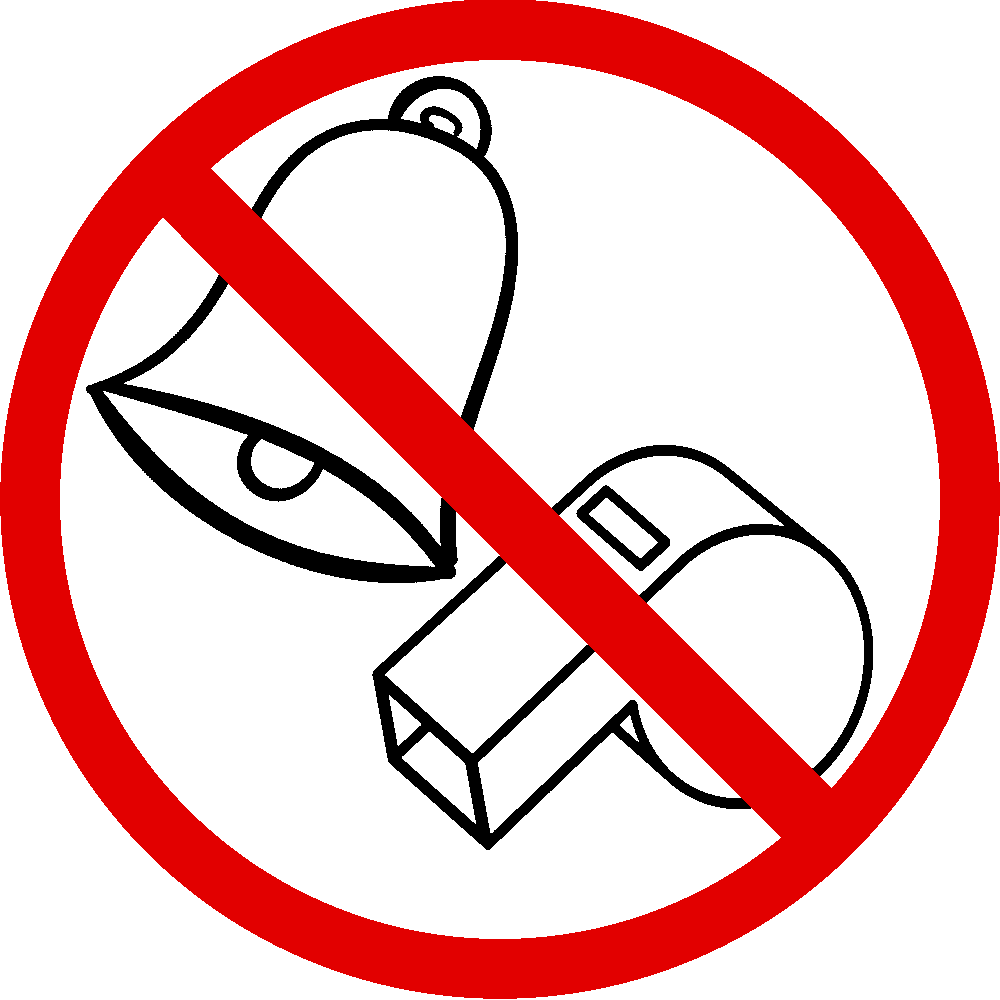
\includegraphics[width=6cm]{sign.png}\\
\makebox[33mm]{}\textbf{Figure 1}
\makebox[62mm]{}\textbf{Figure 2}
\end{figure}


\begin{thebibliography}{42}
\bibitem{ADS} Kurtz M., Eichhorn G., Accomazzi A., et al., 2000, A\&AS, 143, 41
\bibitem{ADS2} Chyla R., Accomazzi A., Holachek A., et al., 2015, ASP Conf. series, 495, 401; arXiv:1503.05881
\bibitem{ADSnew} \url{https://ui.adsabs.harvard.edu}
\bibitem{Obituary} \url{https://adsabs.github.io/blog/ave-atque-vale}
\end{thebibliography}

\end{document}